
\documentclass[letterpaper,12pt]{article}
\usepackage{tabularx} % extra features for tabular environment
\usepackage{amsmath}  % improve math presentation
\usepackage{float}
\usepackage{pdfpages}
\usepackage{cite}
\usepackage{multicol}
\usepackage{graphicx} % takes care of graphic including machinery
\graphicspath{ {./figures/} }
%\usepackage[margin=1in,letterpaper]{geometry} % decreases margins
%\usepackage{cite} % takes care of citations
\usepackage[final]{hyperref} % adds hyperlinks inside the generated pdf file
\hypersetup{
    colorlinks=true,       % false: boxed links; true: colored links
    linkcolor=blue,        % color of internal links
    citecolor=blue,        % color of links to bibliography
    filecolor=magenta,     % color of file links
    urlcolor =blue         
}


\usepackage{fancyhdr}


\title{

\vspace*{0.5in}
\textbf{Fall 2022 EE361 \\ HW1}
\vspace*{0.25in}
}

\author{Ahmet Akman 2442366\\
       } \date{\today}


\begin{document}



\maketitle

\tableofcontents
\newpage
\section{D1)}
The wye connected circuit is constructed in Simulink environment. $R_L$ and \(L_L\) values are selected as 28\(\Omega\) and 38mH respectively, since my student number ends with 6.
\section{D2)}
Simulation is run and the results are obtained.
\subsection{a)}
\(V_{line-line}\) and \(V_{phase}\) are presented in Figure \ref*{D2a} 
\begin{figure}[H]
    \centering
    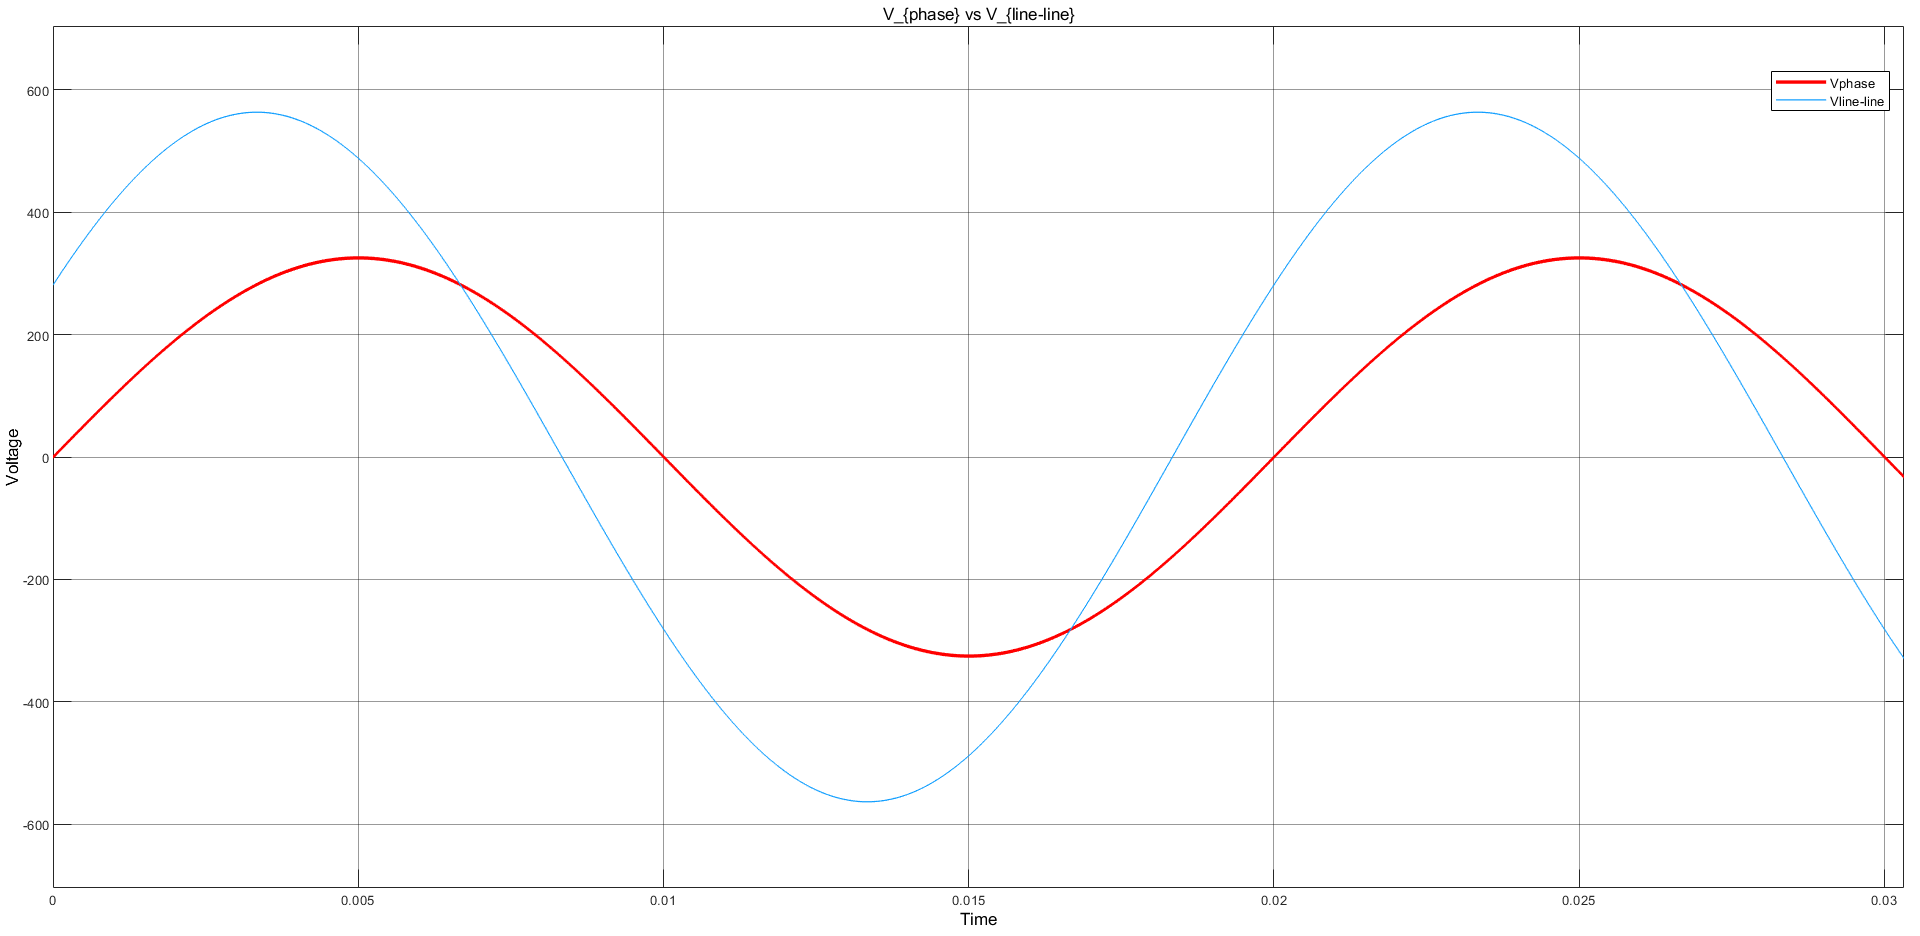
\includegraphics[width = 1\textwidth]{2a.png}
    \caption{\(V_{line-line}\) and \(V_{phase}\) vs Time}
    \label{D2a}
\end{figure} 
\subsection{b)}
\(I_{line}\) and \(I_{phase}\) are presented in Figure \ref*{D2b} 
\begin{figure}[H]
    \centering
    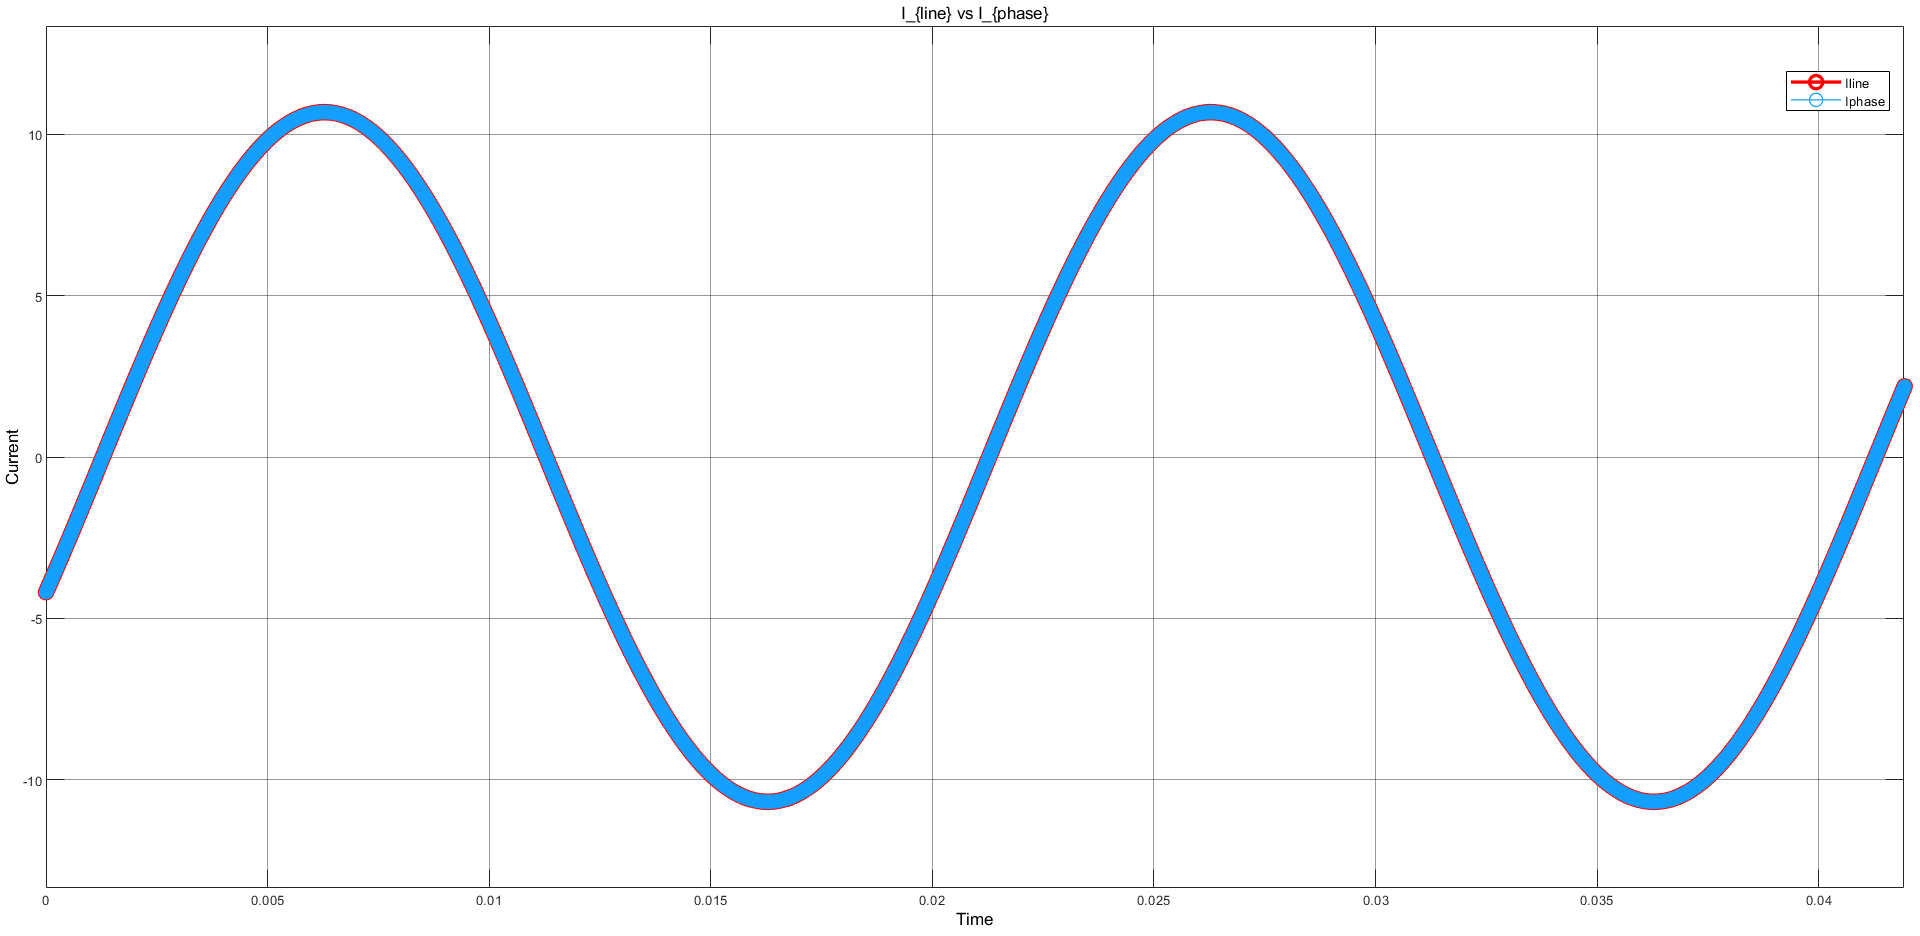
\includegraphics[width = 1\textwidth]{2b.png}
    \caption{\(I_{line}\) and \(I_{phase}\) vs Time}
    \label{D2b}
\end{figure} 
\subsection{c)}
All three phase currents are shown in Figure \ref*{D2c} 
\begin{figure}[H]
    \centering
    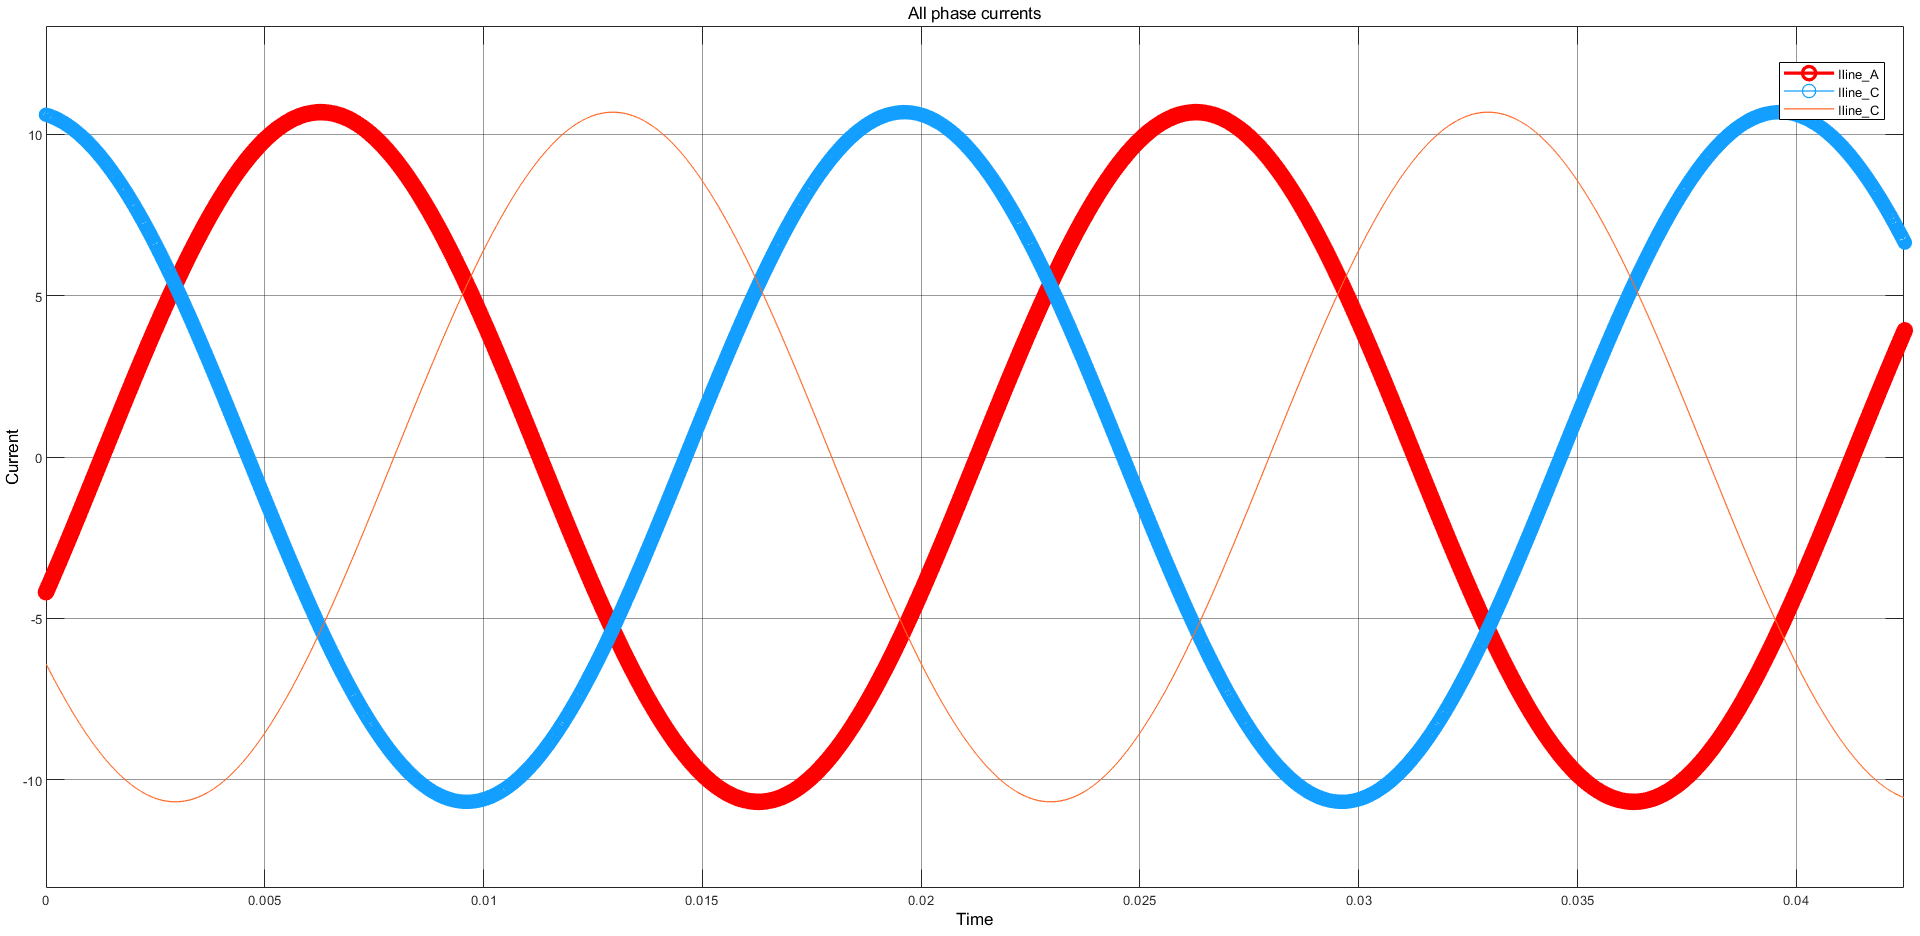
\includegraphics[width = 1\textwidth]{2c.png}
    \caption{All three phase currents vs Time}
    \label{D2c}
\end{figure} 
\subsection{d)}
\(I_{phase}\) and \(V_{phase}\) are presented in Figure \ref*{D2b} 
\begin{figure}[H]
    \centering
    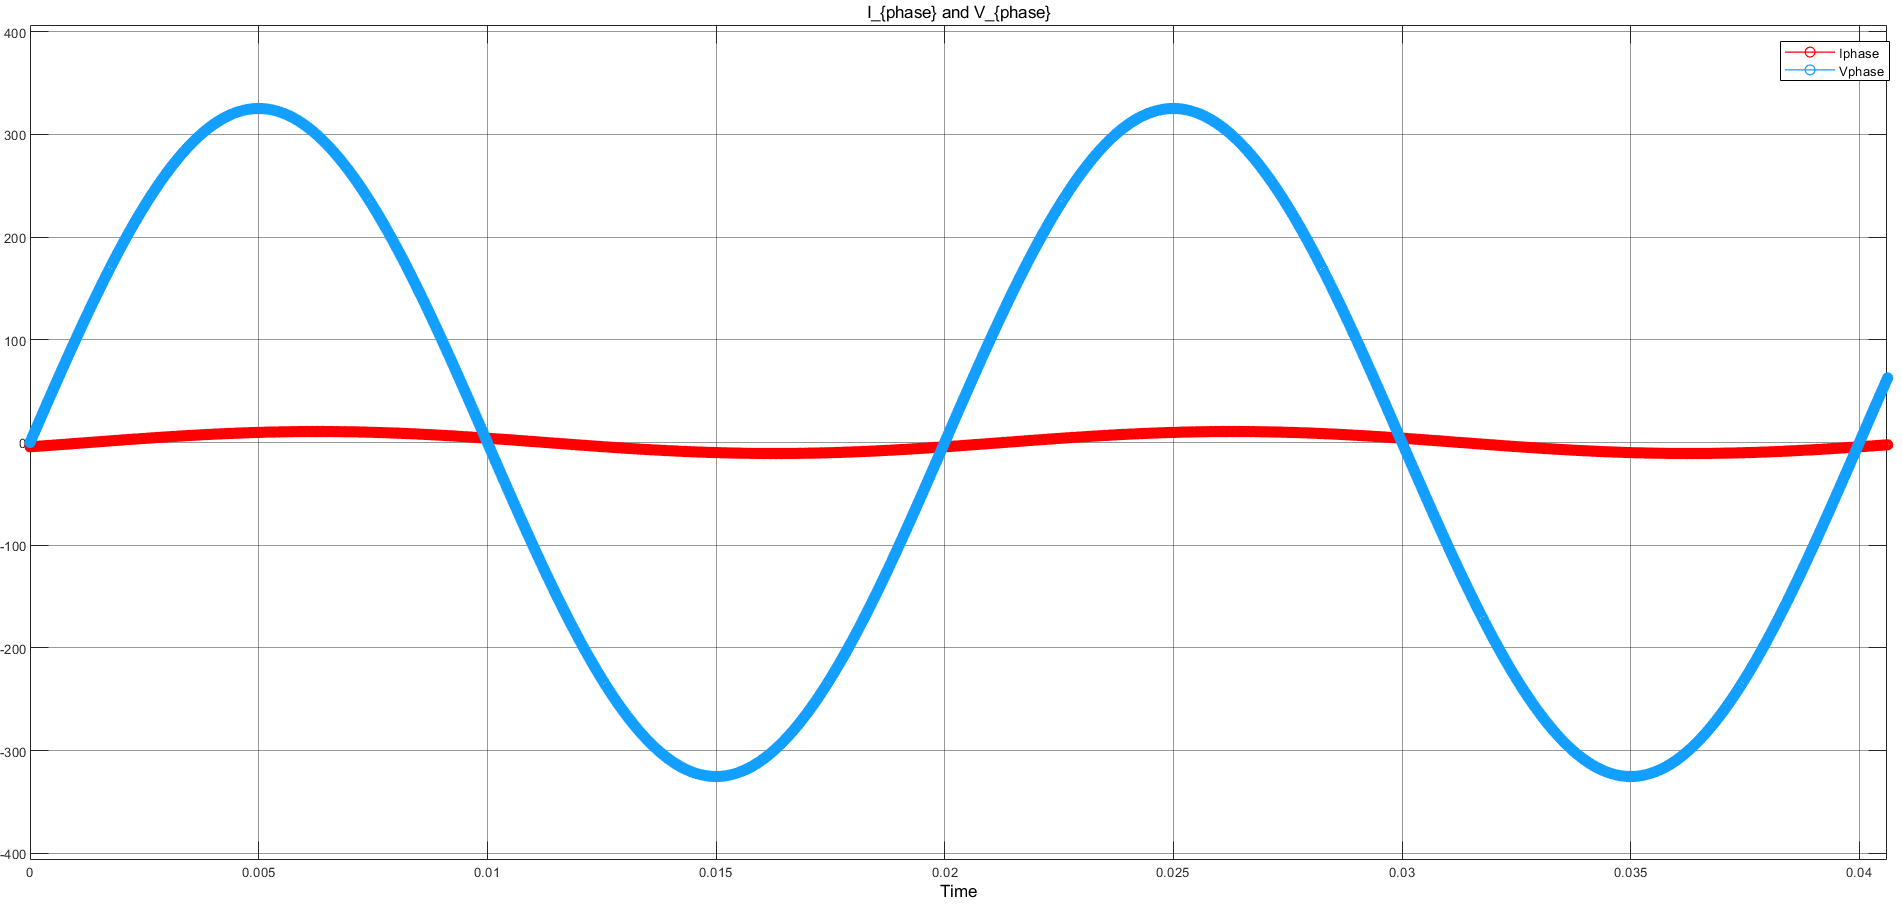
\includegraphics[width = 1\textwidth]{2d.png}
    \caption{\(I_{phase}\) and \(V_{phase}\) of the wye-connected system vs Time}
    \label{D2d}
\end{figure} 
\section{D3)}
The instantaneous power is calculated according to the following expression.
\[
p(t) = v(t) \times i(t)    
\]

When this calculation is done on Simulink, plot given in Figure \ref*{D3}
\begin{figure}[H]
    \centering
    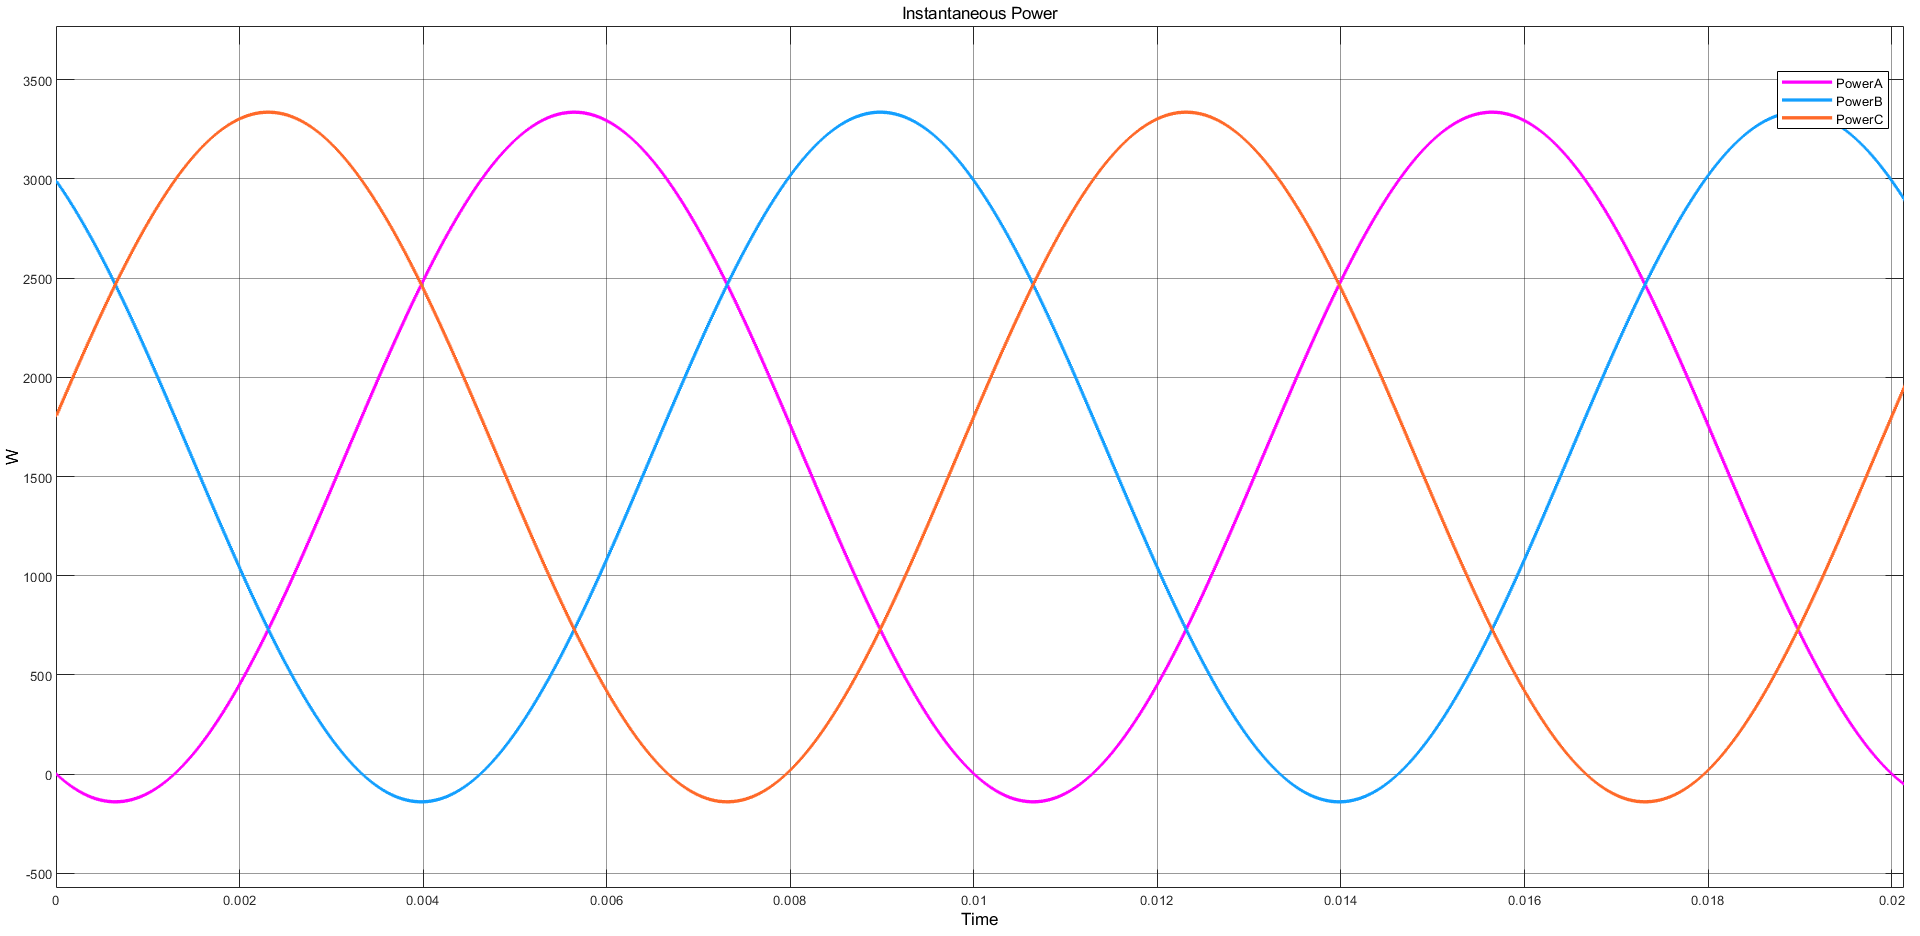
\includegraphics[width = 1\textwidth]{3.png}
    \caption{3-phase instantaneous power}
    \label{D3}
\end{figure}


\section{D4)}
In this section three phase instantaneous power is measured using 2 voltmeters and 2 ampermeters according to the \textbf{two wattmeter method} described in section B/V. .

\subsection{a)}

The Simulink screenshot of the setup is given in Figure \ref*{D4a}.

\begin{figure}[H]
    \centering
    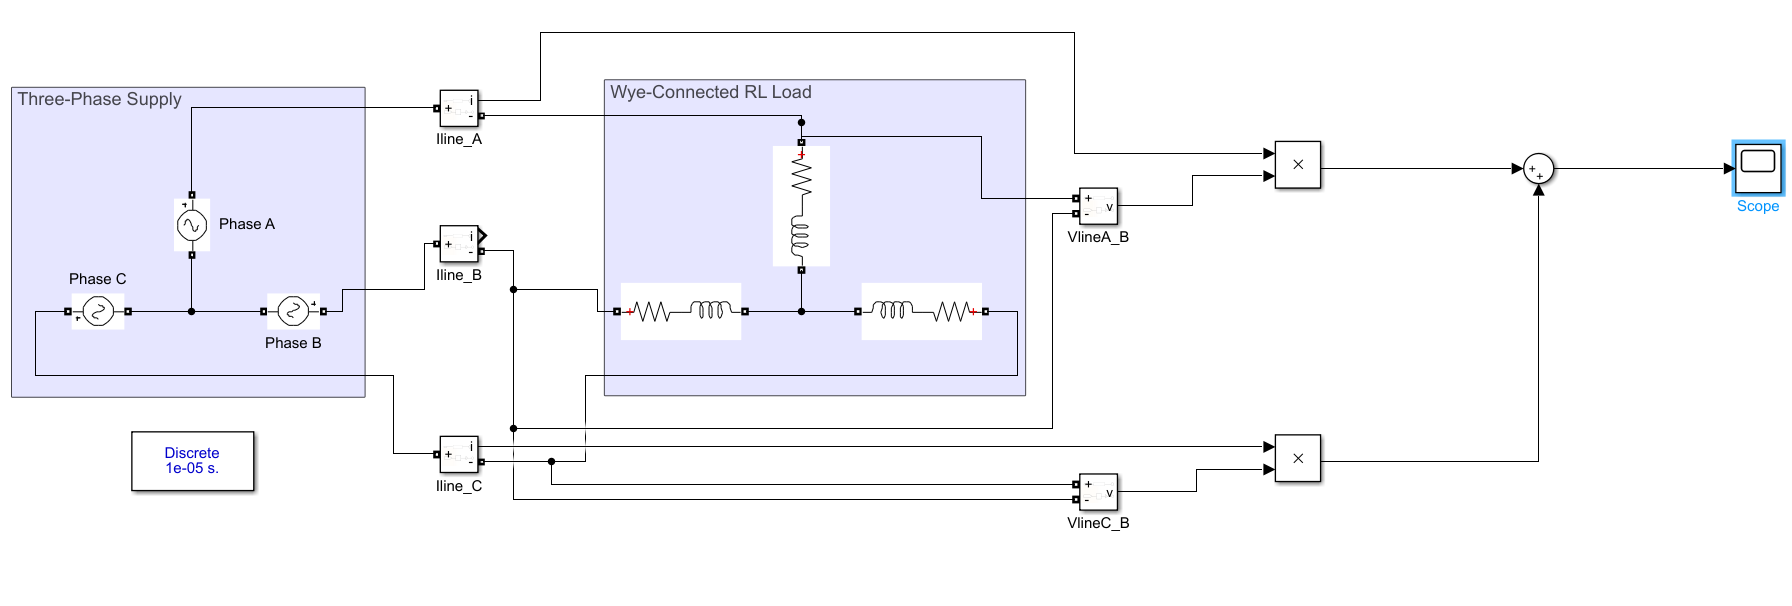
\includegraphics[width = 1\textwidth]{4a.png}
    \caption{Simulink setup for two wattmeter method.}
    \label{D4a}
\end{figure} 
\subsection{b)} 
The result is obtained from the scopes and shown in Figure \ref*{D4b}
\begin{figure}[H]
    \centering
    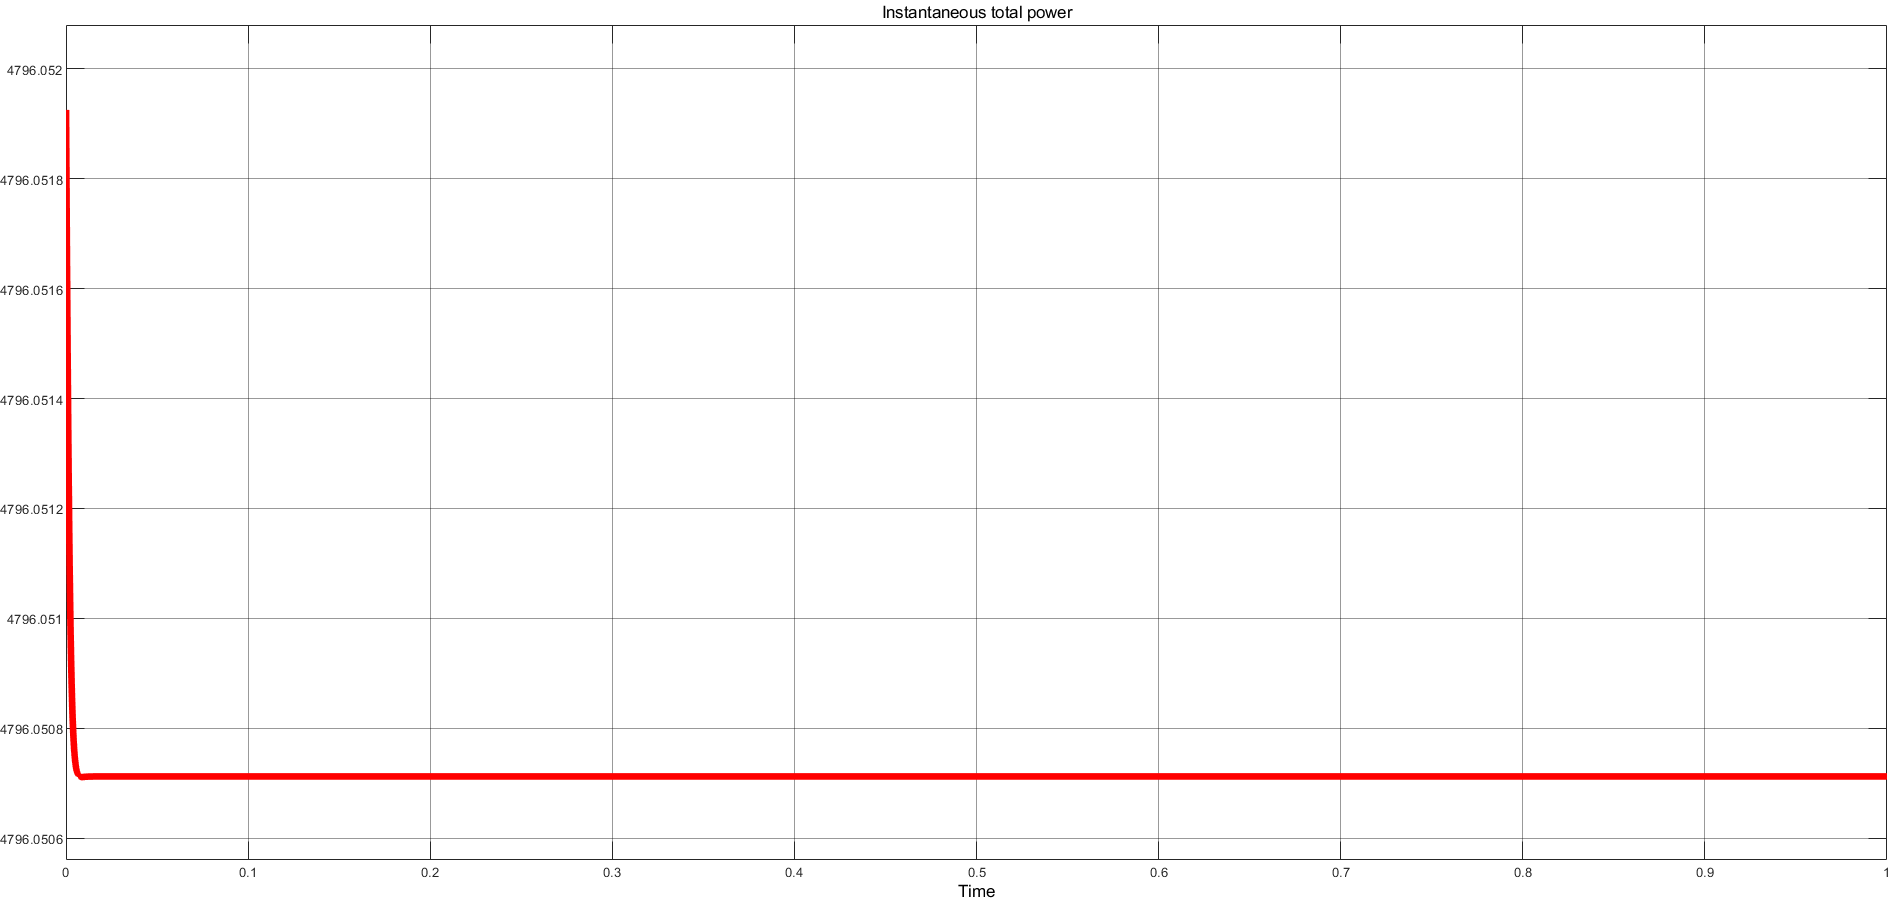
\includegraphics[width = 1\textwidth]{4b.png}
    \caption{Total instantaneous power from two wattmeter}
    \label{D4b}
\end{figure}


\section{D5)}
The phase angle is calculated from the plot given in section D5)d). The time difference between the peaks of the signals are obtained as 0.00125 seconds. The phase angle is calculated as follows.
\begin{equation}
    \begin{split}
        \phi &= 360 \times f \times \Delta t\\
        22.5 &= 360 \times 50 \times 0.00125
    \end{split}
\end{equation}
This phase angle may deviate from the actual value since the peak values are picked up by hand from the plot. Thus the power factor is obtained as 0.9238 . The power is calculated as follows;
\begin{equation}
    \begin{split}
        V_{line-line} &= 398.3717 V_{rms}\\
        So; V_{phase} &= 230 V_{rms}\\
        I_{line} &= 7.55  A_{rms}\\
        \textrm{Thus the single phase apparent power is obtained as  } \\
        \approx & 1736.5\\
        \textrm{As we have found the power factor   we can deduce} & \textrm{complex power as:  } \\
         1604.1787 W &+ 664.8631 VAR \\
        \textrm{Lastly the three phase complex power: } \\
         4812.5361 W & + 1994.5893 VAR .   
    \end{split}
\end{equation} 


\section{D6)}
The values of the load resistance and inductance are doubled for just Phase-A. When the all phase current and voltages measured it is observed that for Phase-A voltage increases and the Phase-A current decreases.
\begin{figure}[H]
    \centering
    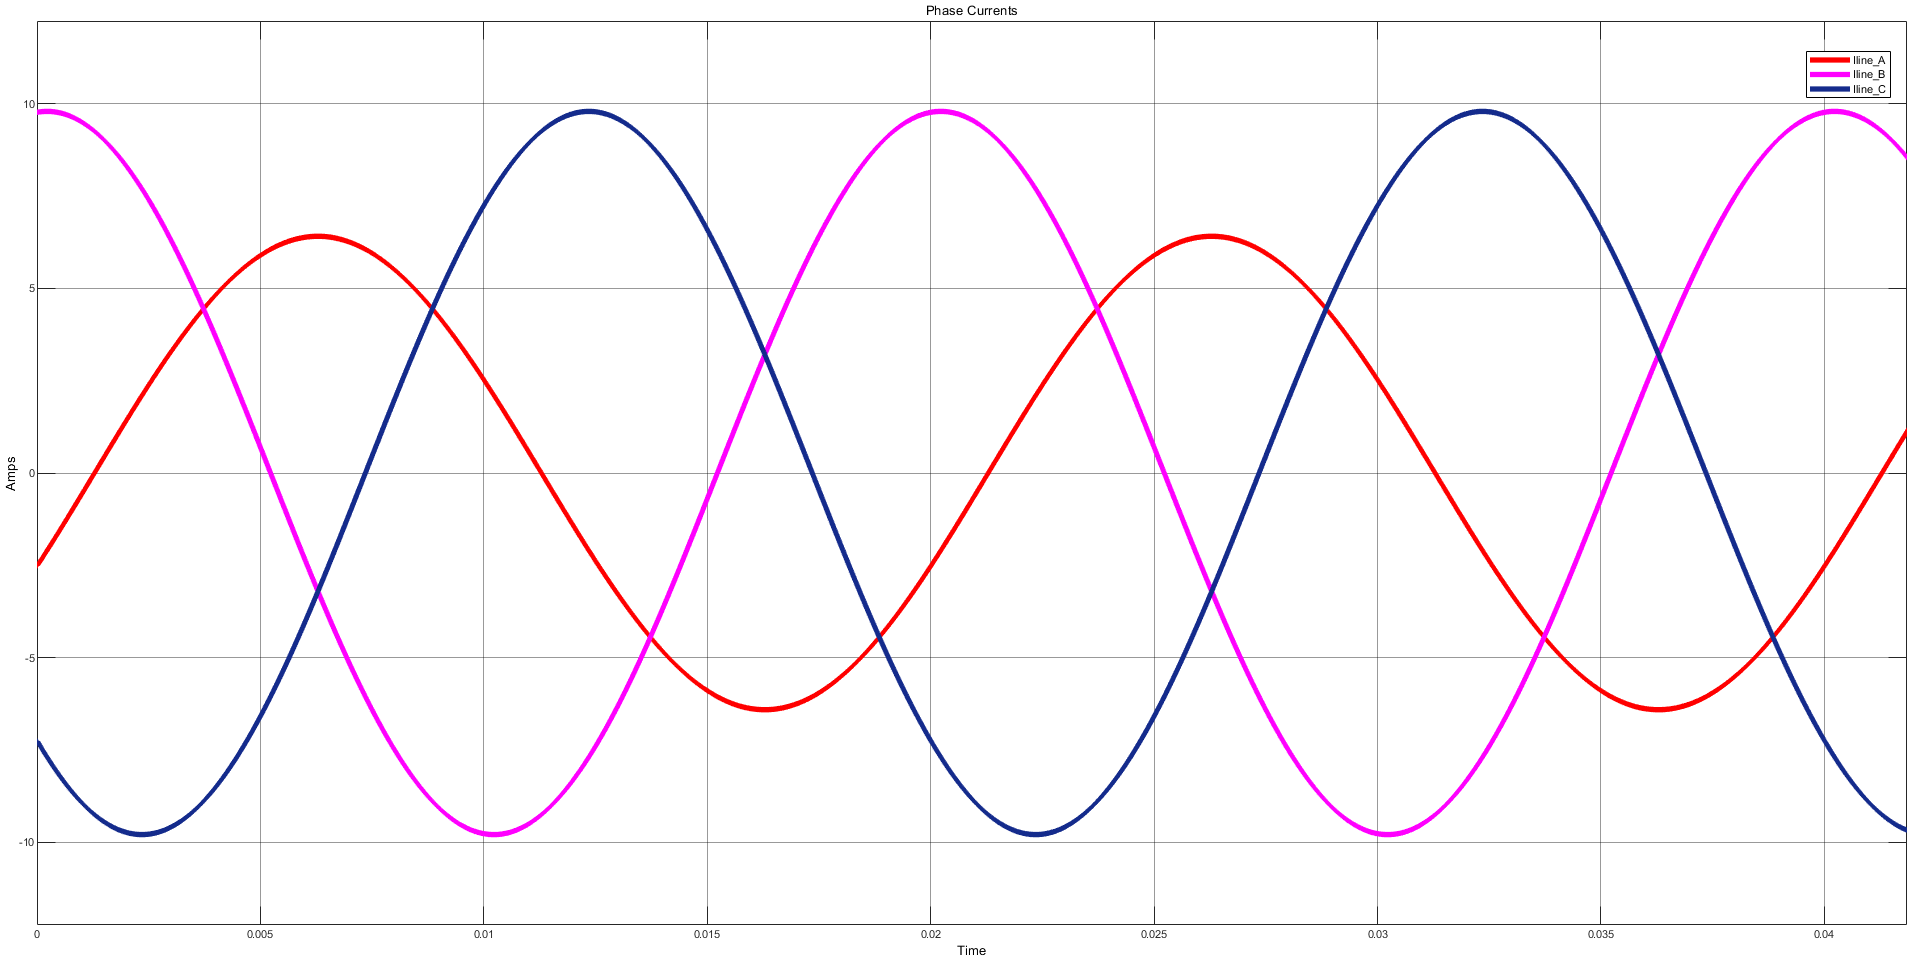
\includegraphics[width = 1\textwidth]{6_1.png}
    \caption{Unbalanced load phase currents}
    \label{D6_1}
\end{figure}
\begin{figure}[H]
    \centering
    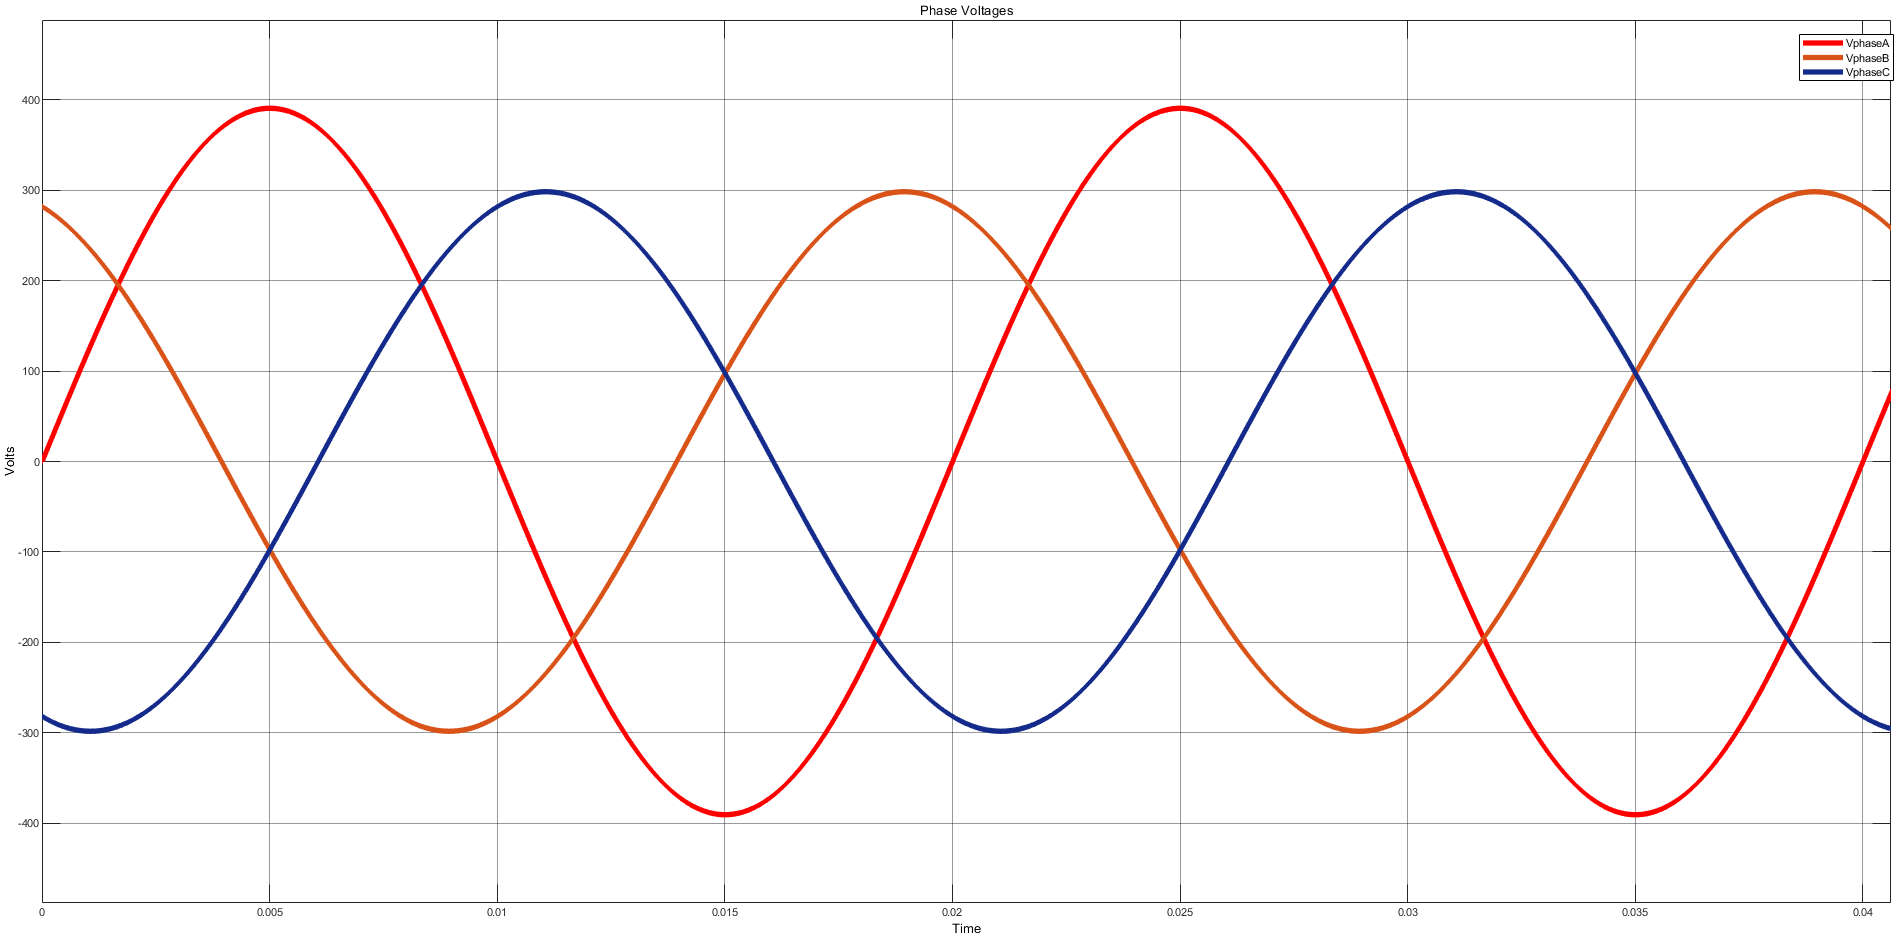
\includegraphics[width = 1\textwidth]{6_2.png}
    \caption{Unbalanced load phase voltages}
    \label{D6_2}
\end{figure}


\section{D7)}
The connection of the load is switched from wye to delta. The resultant configuration is given in Figure \ref*{D7_ss} .
\begin{figure}[H]
    \centering
    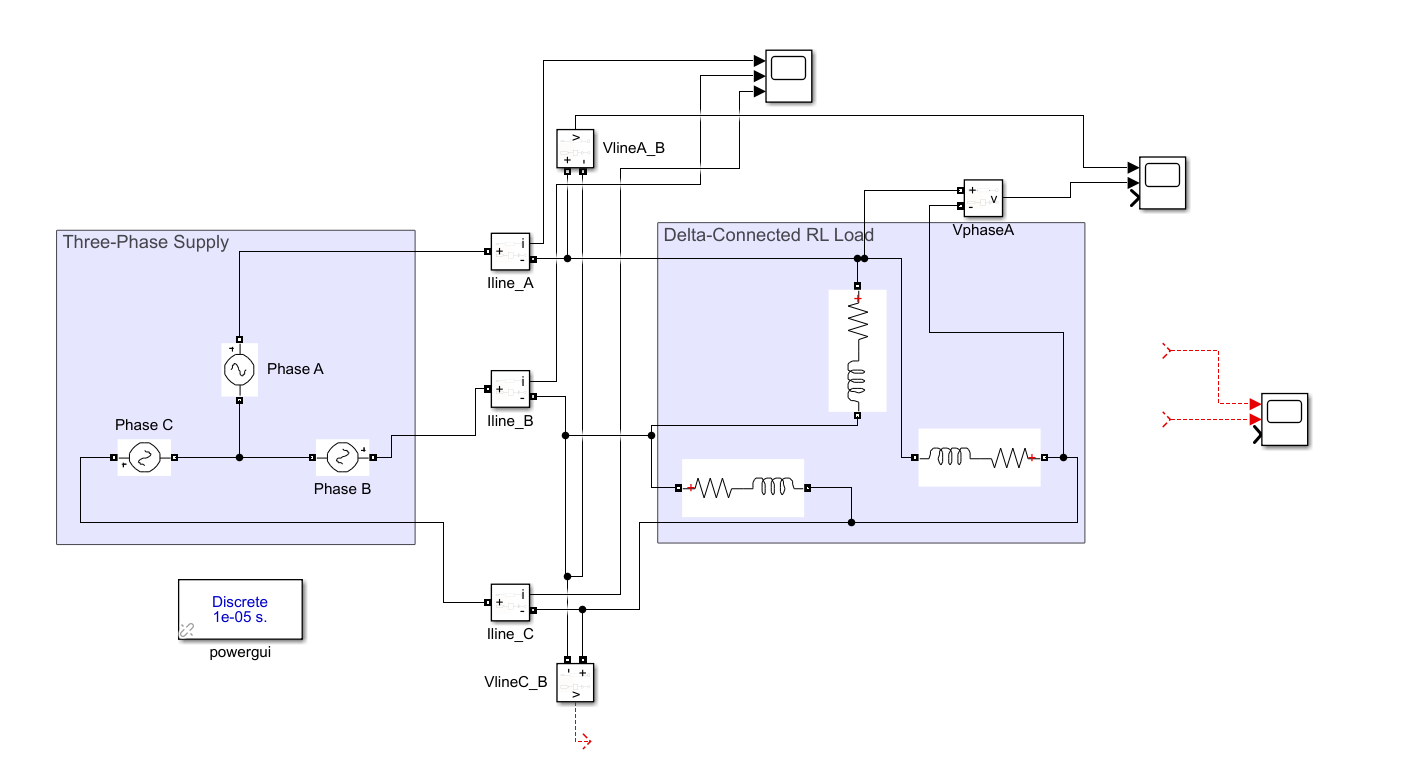
\includegraphics[width = 1\textwidth]{7_ss.png}
    \caption{\(\Delta\) connected load configuration in Simulink}
    \label{D7_ss}
\end{figure}

\subsection{a)}
\(V_{line-line}\) and \(V_phase\) versus time is plotted and given in Figure \ref*{D7a}

\begin{figure}[H]
    \centering
    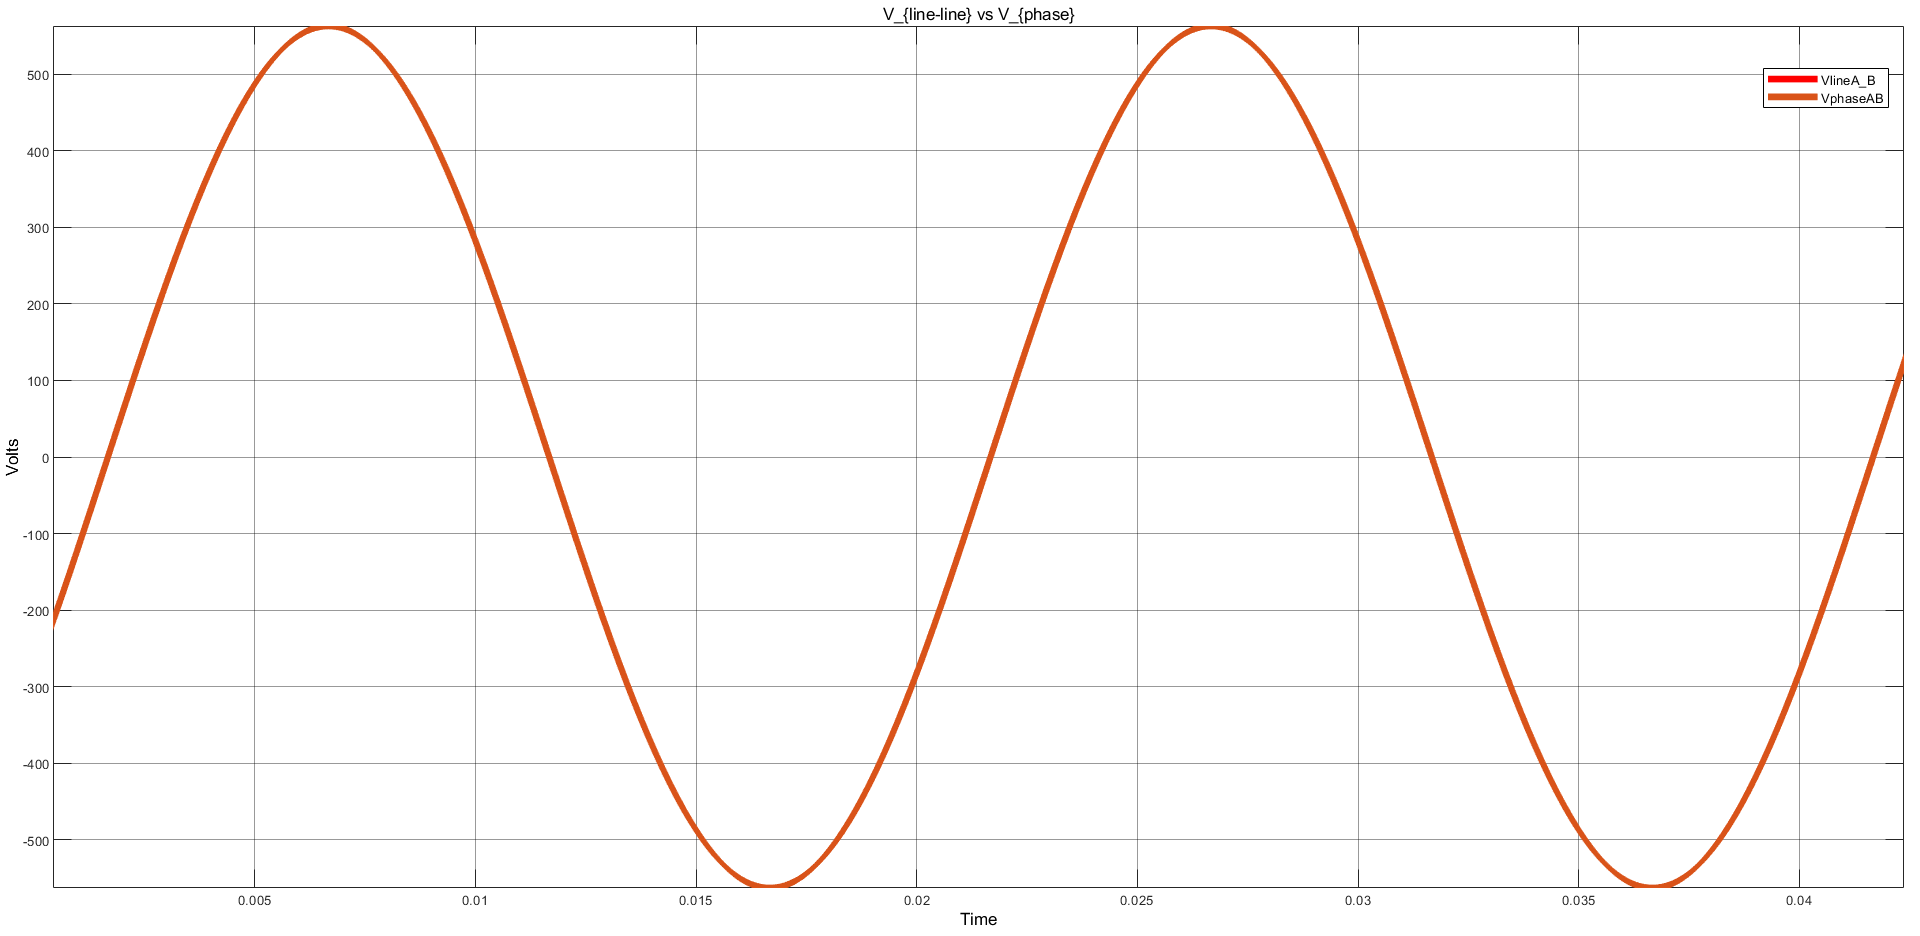
\includegraphics[width = 1\textwidth]{7_1.png}
    \caption{\(V_{line-line}\) , \(V_{phase}\) vs Time }
    \label{D7a}
\end{figure}

\subsection{b)}
\(I_{line}\) and \(I_phase\) versus time is plotted and given in Figure \ref*{D7b}

\begin{figure}[H]
    \centering
    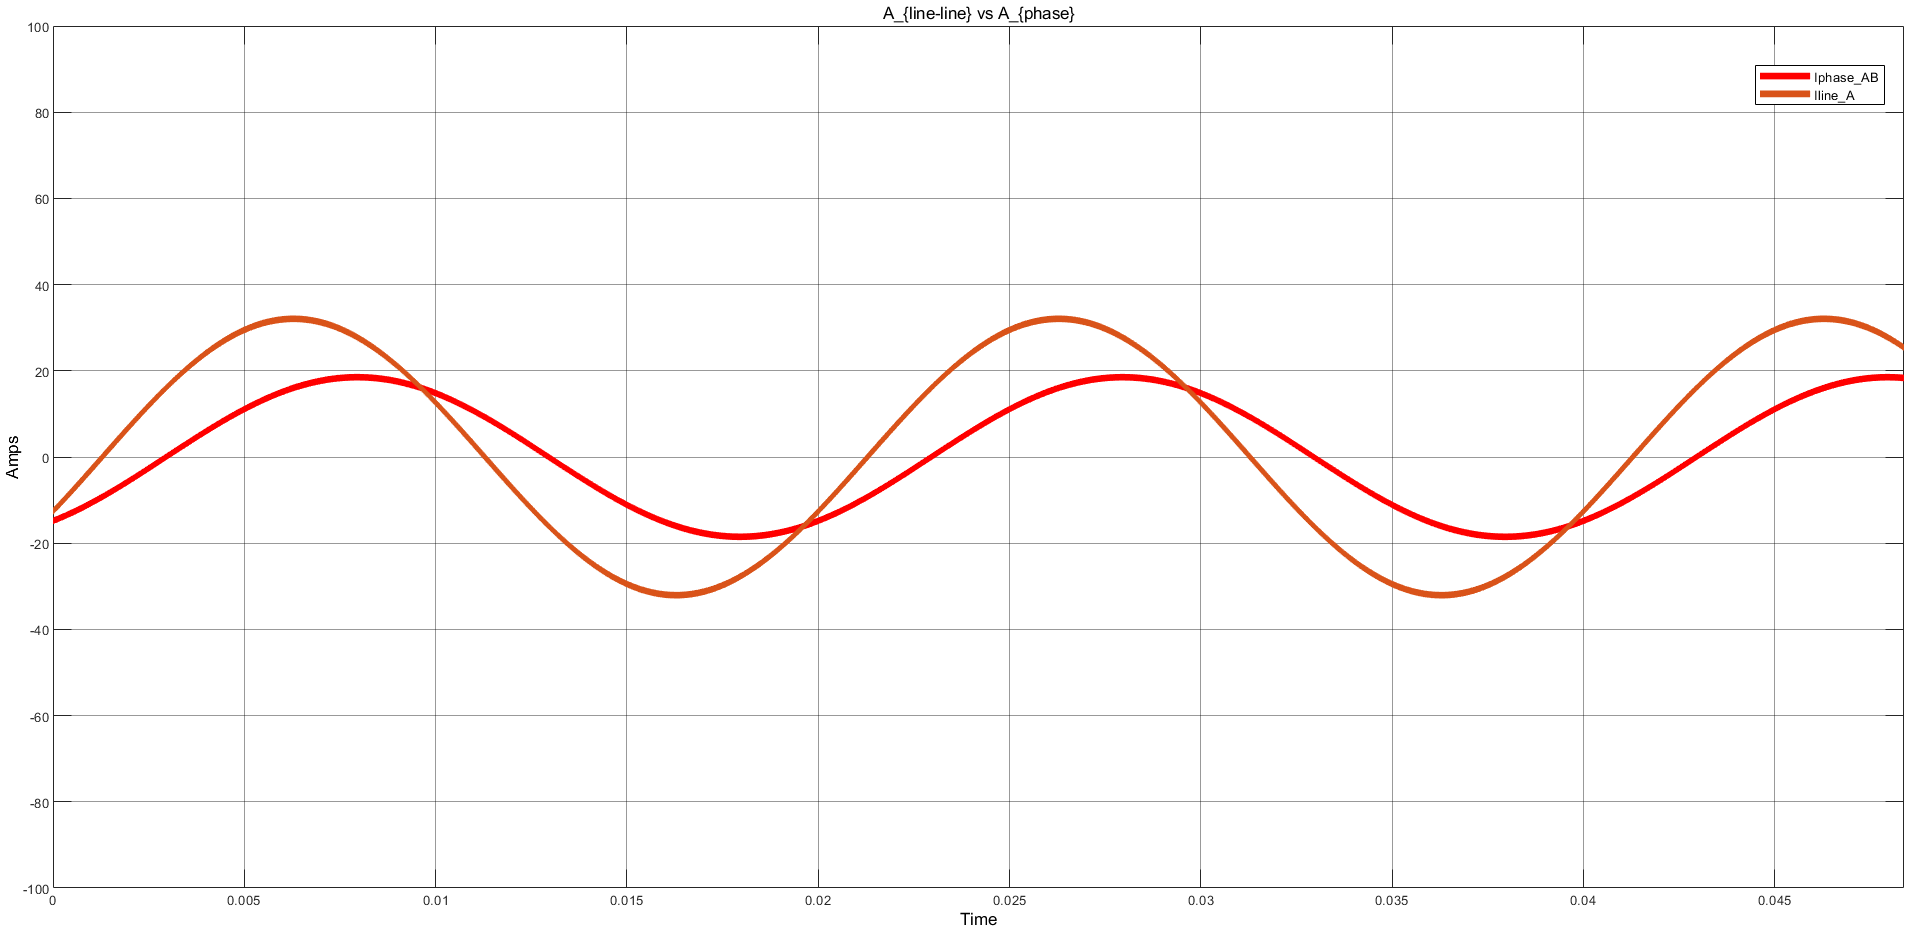
\includegraphics[width = 1\textwidth]{7_3.png}
    \caption{\(I_{line}\) , \(I_{phase}\) vs Time }
    \label{D7b}
\end{figure}
\subsection{c)}
\(I_phase\) and \(V_phase\) versus time is plotted for \(\Delta\) connected load and given in Figure \ref*{D7c}.

\begin{figure}[H]
    \centering
    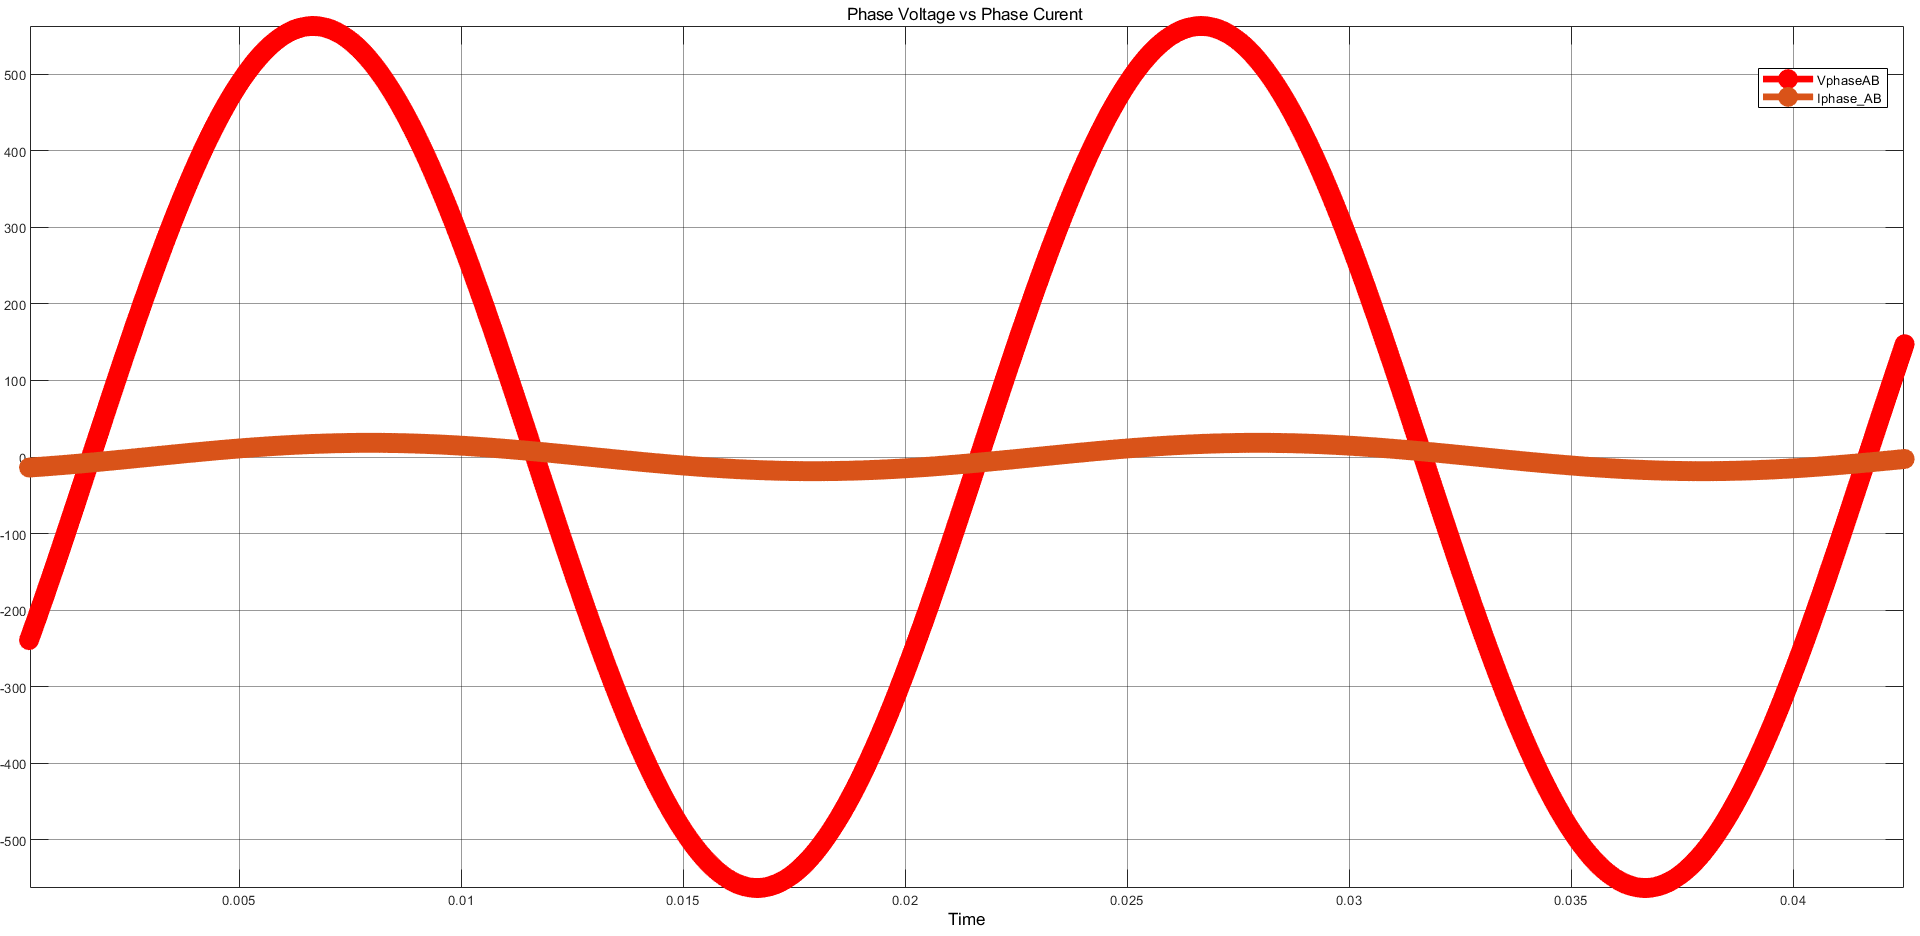
\includegraphics[width = 1\textwidth]{7_2.png}
    \caption{\(I_{phase}\) , \(V_{phase}\) of \(\Delta\) connected system. }
    \label{D7c}
\end{figure}


\section{D8)}
The phase angle is calculated from the plot given in section D7)c). The time difference between the peaks of the signals are obtained as 0.00125 seconds. The phase angle is calculated as follows.
\begin{equation}
    \begin{split}
        \phi &= 360 \times f \times \Delta t\\
        22.5 &= 360 \times 50 \times 0.00125
    \end{split}
\end{equation}
Thus the power factor is obtained as 0.9238 (same with the wye-connected configuration) . The power is calculated as follows;
\begin{equation}
    \begin{split}
        V_{line-line} &= 398.3717 V_{rms}\\
        So; V_{phase} &= 230 V_{rms}\\
        I_{line-line} &= 22.06  A_{rms}\\ 
        \textrm{From this information 3 phase }& \textrm{ apparent power directly calculated as} \\
        398.3717 \times 22.06 \times \sqrt{3} = &15221.869  \\
        \textrm{Lastly the three phase complex power: } \\
         14061 W & +5824.82  VAR .   
    \end{split}
\end{equation} 
\section{E1)}
It is impossible to get constant instantaneous power with a regular single-phase system. This is duet to the fact that in single-phase there are no other line to balance the sinusoid signal in instantaneous manner.
\section{E2)}
Using wye-connected and \(\Delta\)-connected systems provide an advantage of less wire connection. Since the systems are balanced there are no neutral wires or very thin neutral wires compared to the phase lines. Thus, wye and \(\Delta\)-connected systems reduces cost.

\section{E3)}
In Figure  \ref*{E3} the per-phase representation and the calculations are provided.

\begin{figure}[H]
    \centering
    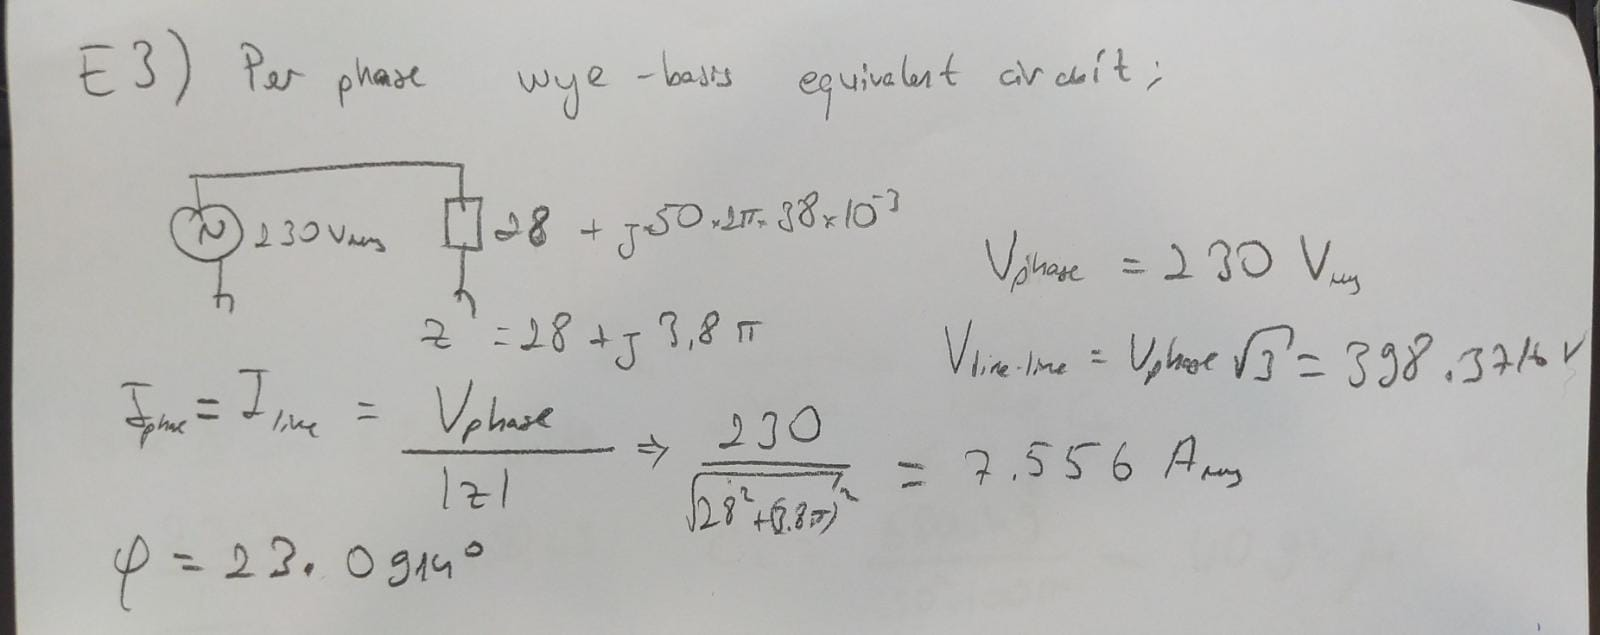
\includegraphics[width = 1\textwidth]{E3.jpeg}
    \caption{Per phase wye-basis calculations }
    \label{E3}
\end{figure}

\section{E4)}
It can be said that the simulation results are quite close to the calculation as expected. 
\section{E5)}
In Figure \ref*{E5} the phasor diagram of the per phase wye-basis circuit is provided.

\begin{figure}[H]
    \centering
    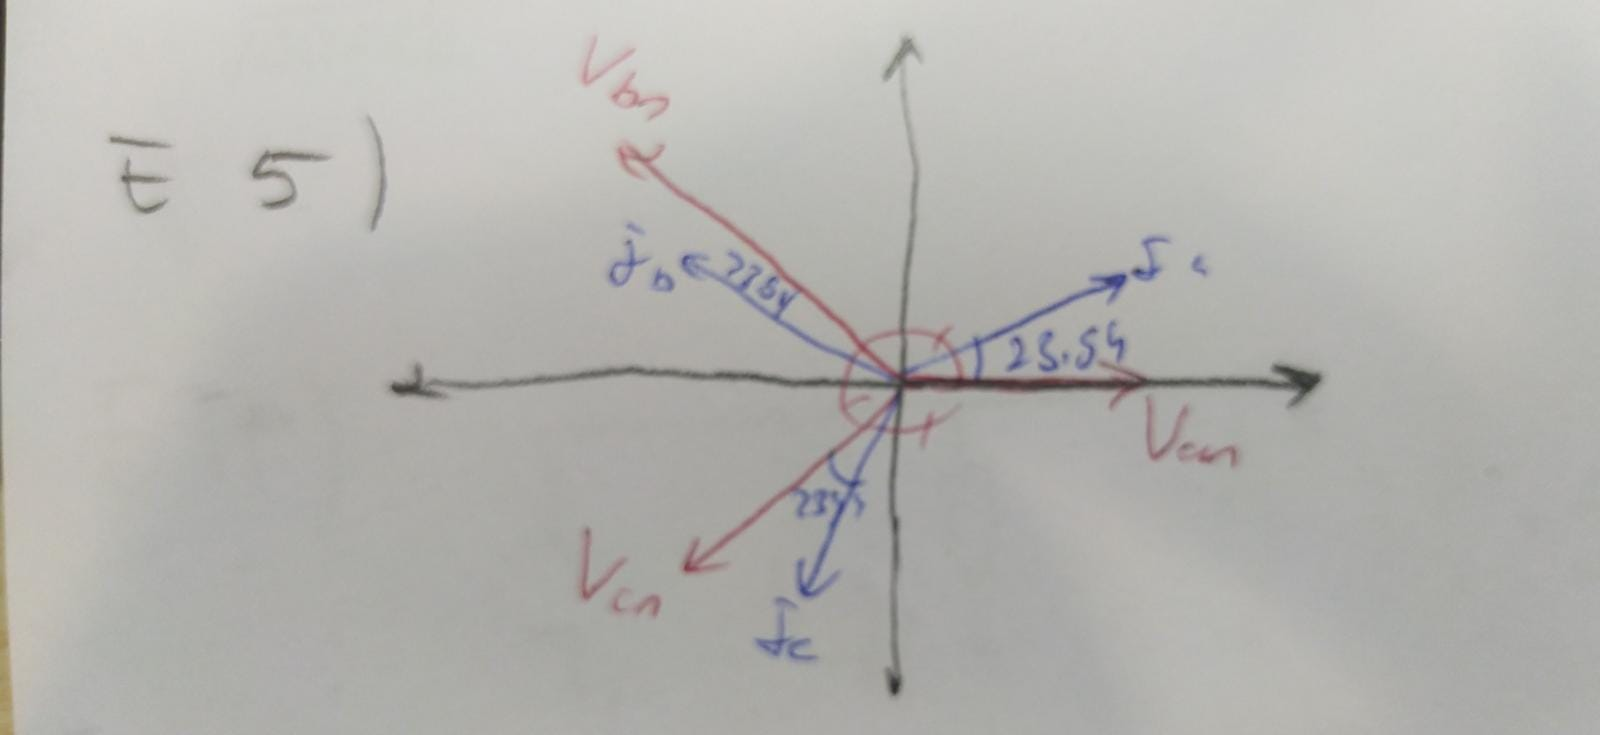
\includegraphics[width = 1\textwidth]{E5.jpeg}
    \caption{Phasor diagram}
    \label{E5}
\end{figure}
\section{E6)}
By comparison it can be said that the results are quite close, however not identical. These devaitations may stemmed from the some non-idealities of my measurement method and my calculation approach. For example some of the significant figures are ignored through my calculations.
\section{E7)}
The wye-basis equivalent circuit is given in Figure \ref*{E7} with the equivalent R and L values.

\begin{figure}[H]
    \centering
    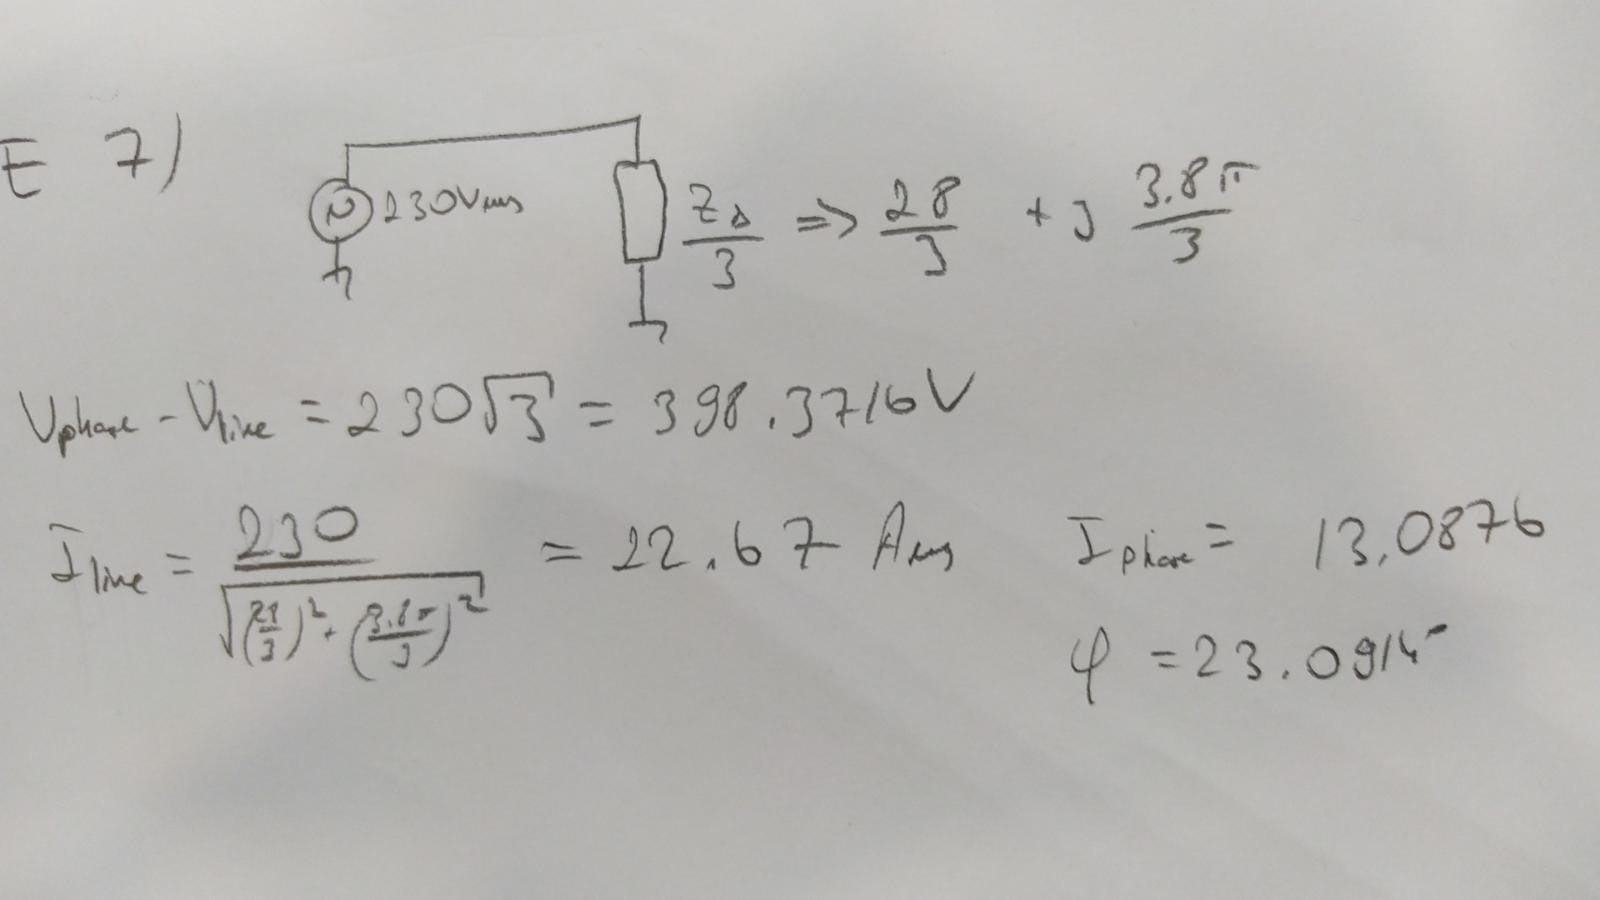
\includegraphics[width = 1\textwidth]{E7.jpeg}
    \caption{Per phase delta-basis calculations }
    \label{E7}
\end{figure}

\section{E8)}
When the line currents calculated with  wye and \(Delta\) connected loads are compared the following statement can be made:
\[
I_{line_\Delta} = \sqrt{3} I_{line_{wye}}    
\]

\section{E9)}
Overall power delivered to the load does change when the RL load connection is changed from wye to \(\Delta\) . Indeed, the Q part is increased significantly.

\section{E10)}
The power factor correction calculations for wye-connected load are given in Figure \ref*{E10}.

\begin{figure}[H]
    \centering
    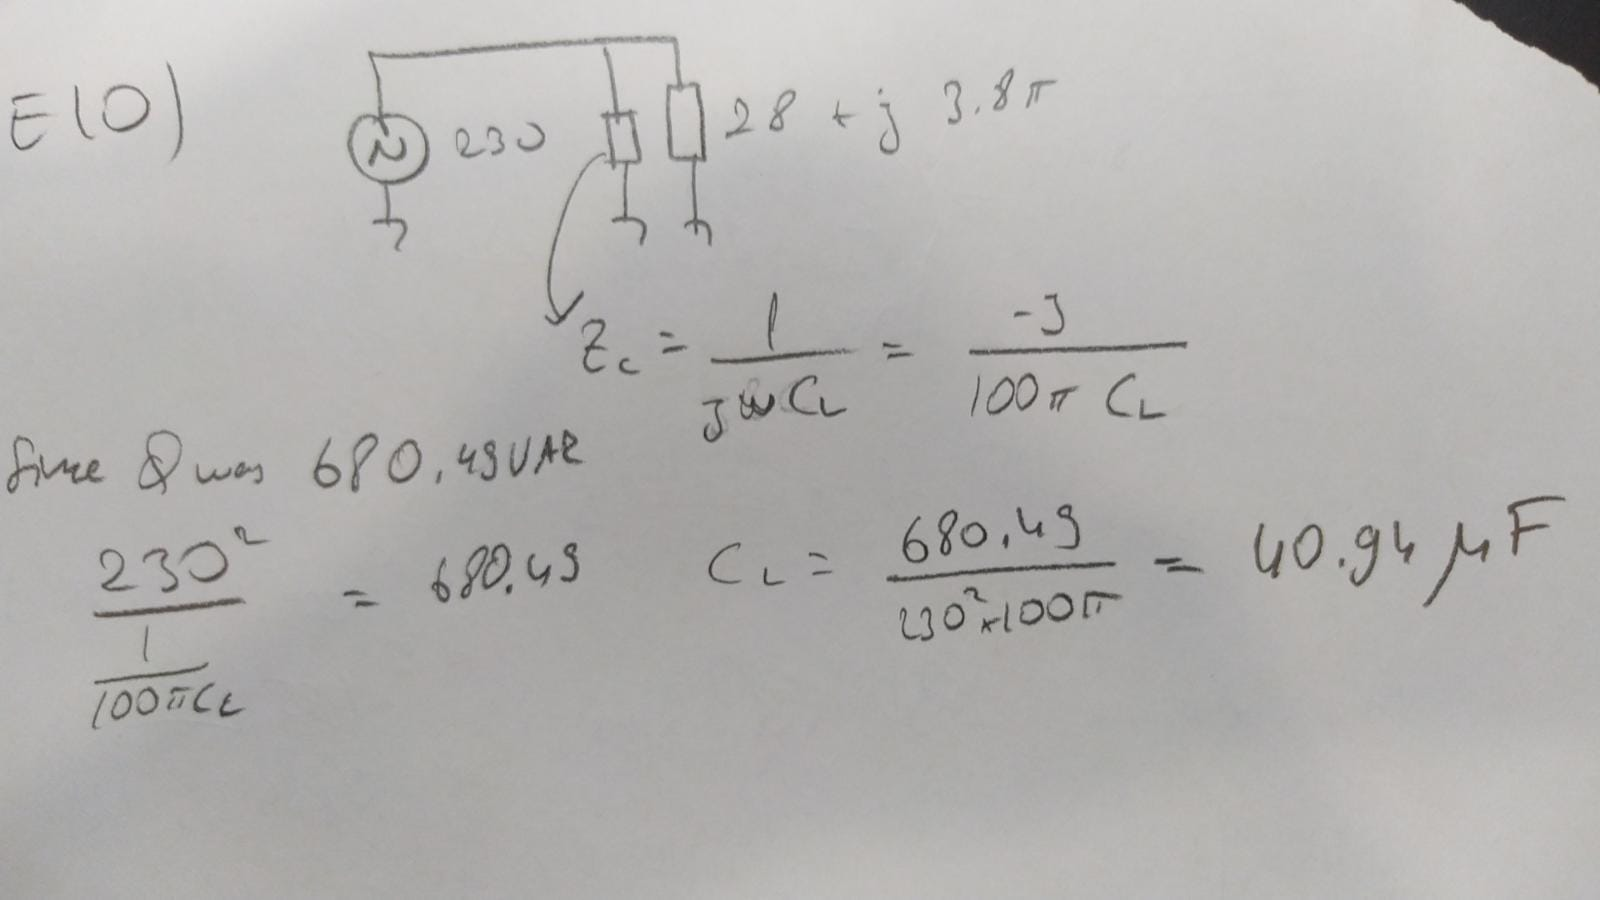
\includegraphics[width = 1\textwidth]{E10.jpeg}
    \caption{Power factor correction for wye-basis}
    \label{E10}
\end{figure}
\section{E11)}
The power factor correction calculations for delta-connected load are given in Figure \ref*{E11}.


\begin{figure}[H]
    \centering
    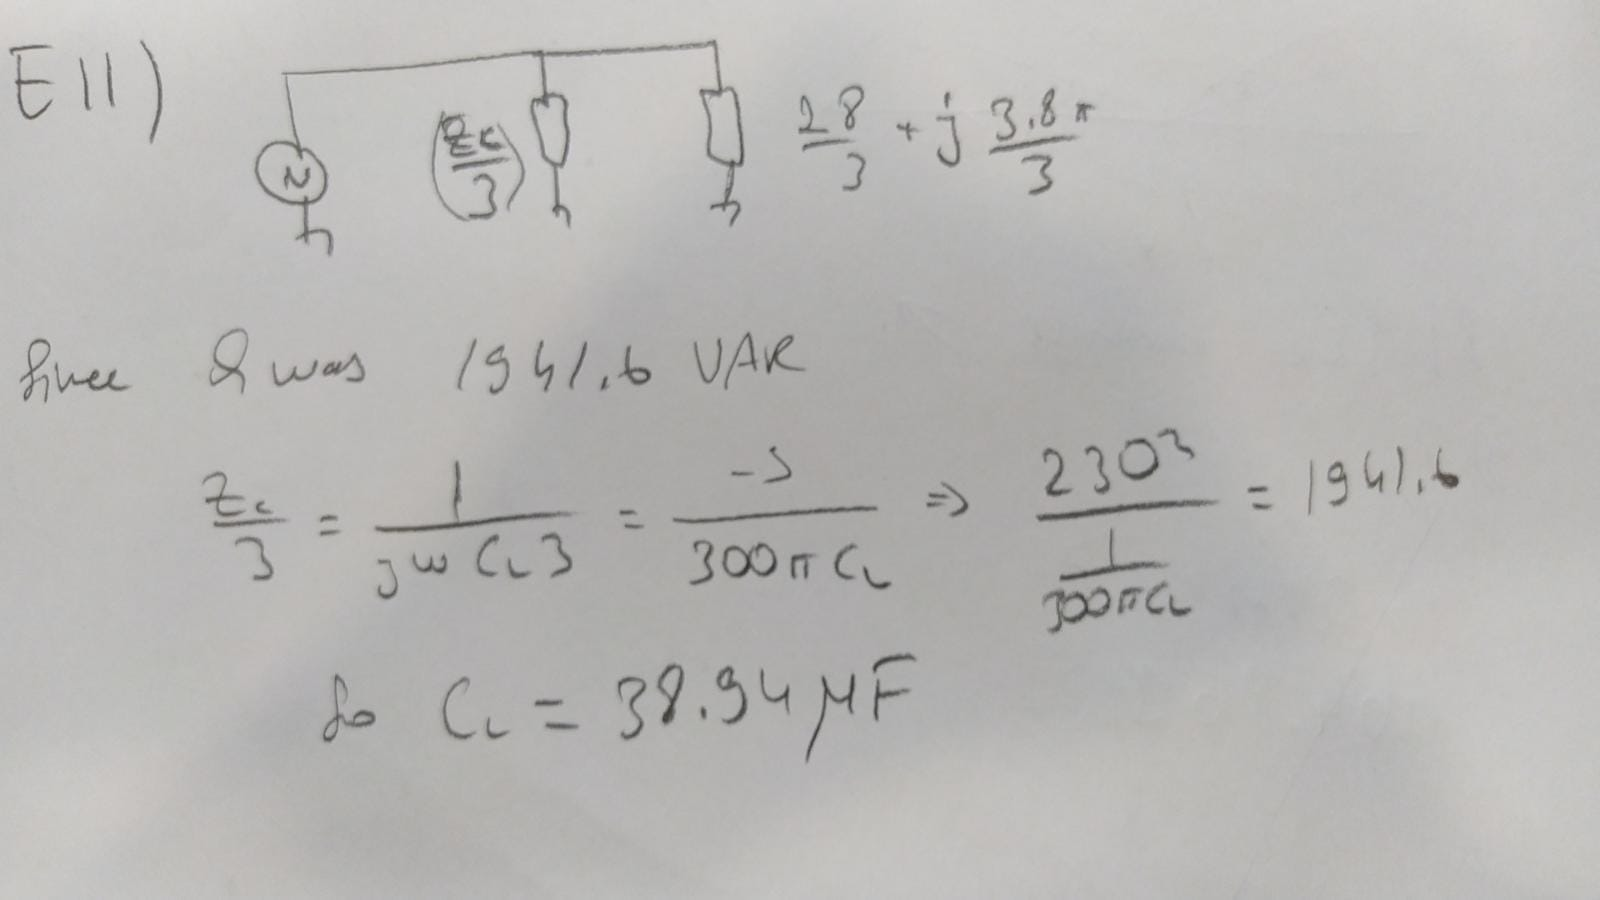
\includegraphics[width = 1\textwidth]{E11.jpeg}
    \caption{Power factor correction calculations for delta-connected load}
    \label{E11}
\end{figure}


\section{Conclusion} In this document results of the first homework of fall semester are presented. 

\end{document}

%%%%%%%%%%%%%%%%%%%%%%   EXAMPLE TABLE   %%%%%%%%%%%%%%%%%%%%%%%%%%%%%%%%
\begin{table}[H]
\begin{center}
    \caption{Resistance reading by color code convention.}
    \vspace{2mm}
    \begin{tabular}{||c | c | c||} 
        \hline
        Color Order & Value & Tolerance \\ [0.5ex] 
        \hline\hline
        Brown / Black / Red / Gold & 1k\( \Omega \) & \( \% \) 5  \\ 
        \hline
        Yellow / Violet / Red / Gold & 4.7k\( \Omega \) & \( \% \) 5   \\
        \hline
        Brown / Grey / Orange / Gold & 18k\( \Omega \) & \( \% \) 5  \\ [1ex] 
        \hline
    \end{tabular}
\end{center}
\end{table}


%%%%%%%%%%%%%%%%%%%%%%   EXAMPLE IMAGE   %%%%%%%%%%%%%%%%%%%%%%%%%%%%%%%%
\begin{figure}[H]
\centering
\includegraphics[width = 0.75\textwidth]{5.png}
\caption{Circuit schematic for step 5}
\end{figure} 

%%%%%%%%%%%%%%%%%%%%%%   EXAMPLE IMAGE FROM PDF   %%%%%%%%%%%%%%%%%%%%%%%%%%%%%%%%
\begin{figure}[H] \centering{
    \includegraphics[scale=0.25]{2a_plot.pdf}}
    \caption{Experiment 2}
\end{figure}